\chapter{Results {\&} Analysis}
\label{chap:resultsanalysis}
In this chapter the results of both experiments, introduced in Chapter \ref{chap:experiment}, are presented and analysed.

\section{Implementation that uses Simple Event Correlators own rule format (regex based)}

\begin{figure}[ht]
\centering
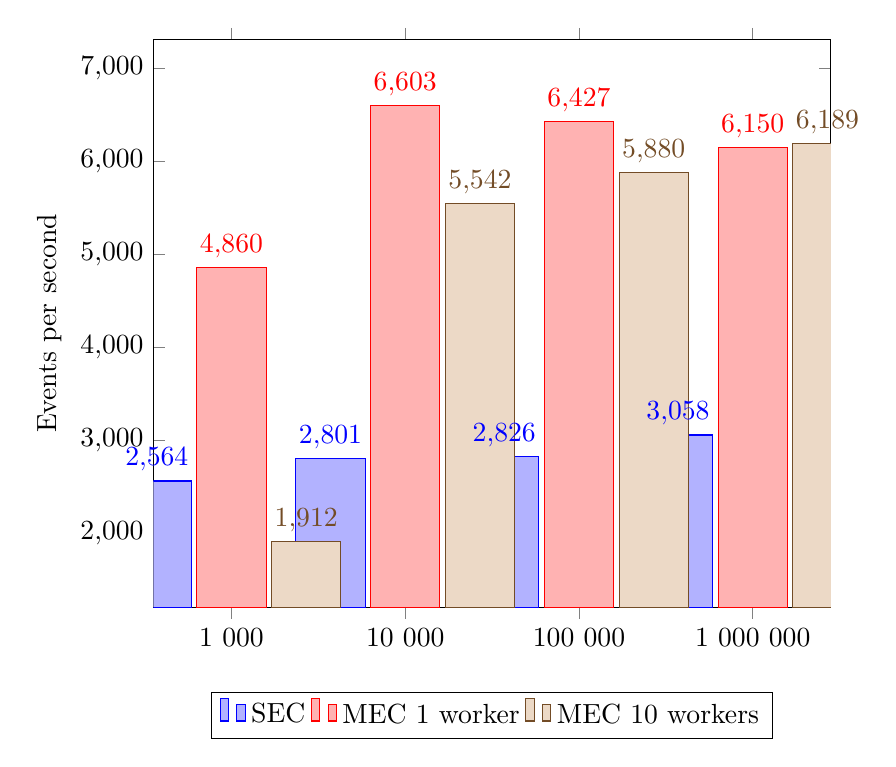
\begin{tikzpicture}
\begin{axis}[
    xtick=data,
	height=250pt,
	ylabel=Events per second,
	enlargelimits=0.15,
	legend style={at={(0.5,-0.15)},
	anchor=north,legend columns=-1},
	ybar,
	bar width=25pt,
	symbolic x coords={1 000, 10 000, 100 000, 1 000 000},
	nodes near coords,
	nodes near coords style={above}
]
\addplot coordinates {(1 000,2564) (10 000,2801) (100 000,2826) (1 000 000,3058)}; % SEC
\addplot coordinates {(1 000,4860) (10 000,6603) (100 000,6427) (1 000 000,6150)}; % MEC1W
\addplot coordinates {(1 000,1912) (10 000,5542) (100 000,5880) (1 000 000,6189)}; % MEC10W
\legend{SEC, MEC 1 worker, MEC 10 workers}
\end{axis}
\end{tikzpicture}
\caption{Baseline dataset}
\label{fig:baseline-perf}
\end{figure}


\begin{figure}[ht]
\centering
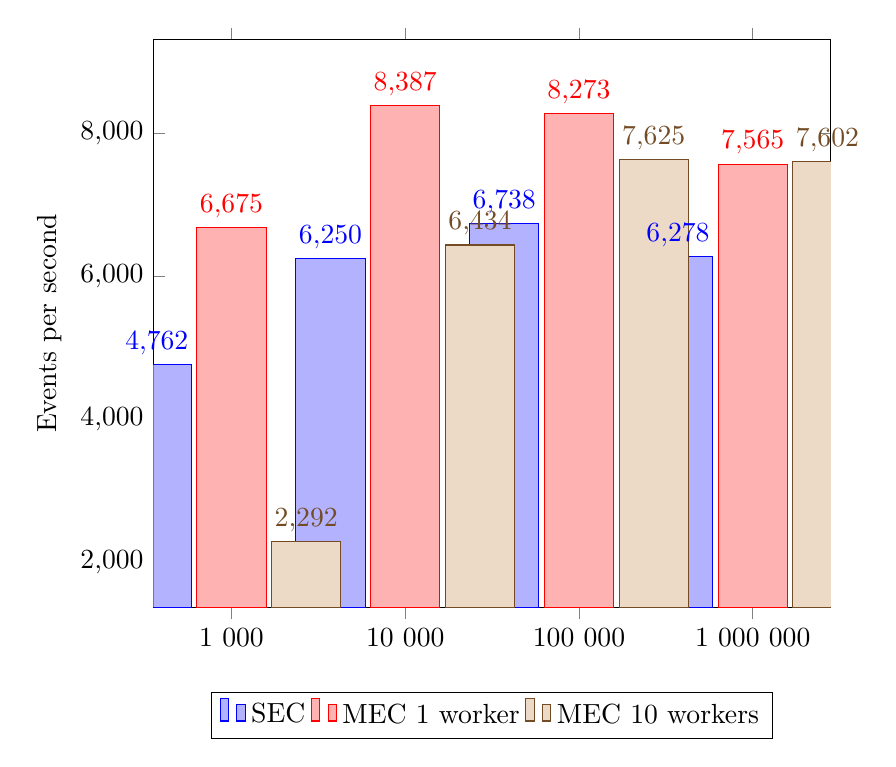
\begin{tikzpicture}
\begin{axis}[
    xtick=data,
	height=250pt,
	ylabel=Events per second,
	enlargelimits=0.15,
	legend style={at={(0.5,-0.15)},
	anchor=north,legend columns=-1},
	ybar,
	bar width=25pt,
	symbolic x coords={1 000, 10 000, 100 000, 1 000 000},
	nodes near coords,
	nodes near coords style={above}
]
\addplot coordinates {(1 000,4762) (10 000,6250) (100 000,6738) (1 000 000,6278)}; % SEC
\addplot coordinates {(1 000,6675) (10 000,8387) (100 000,8273) (1 000 000,7565)}; % MEC1W
\addplot coordinates {(1 000,2292) (10 000,6434) (100 000,7625) (1 000 000,7602)}; % MEC10W
\legend{SEC, MEC 1 worker, MEC 10 workers}
\end{axis}
\end{tikzpicture}
\caption{High signal low noise dataset}
\label{fig:high-signal-low-noise}
\end{figure}


\begin{figure}[ht]
\centering
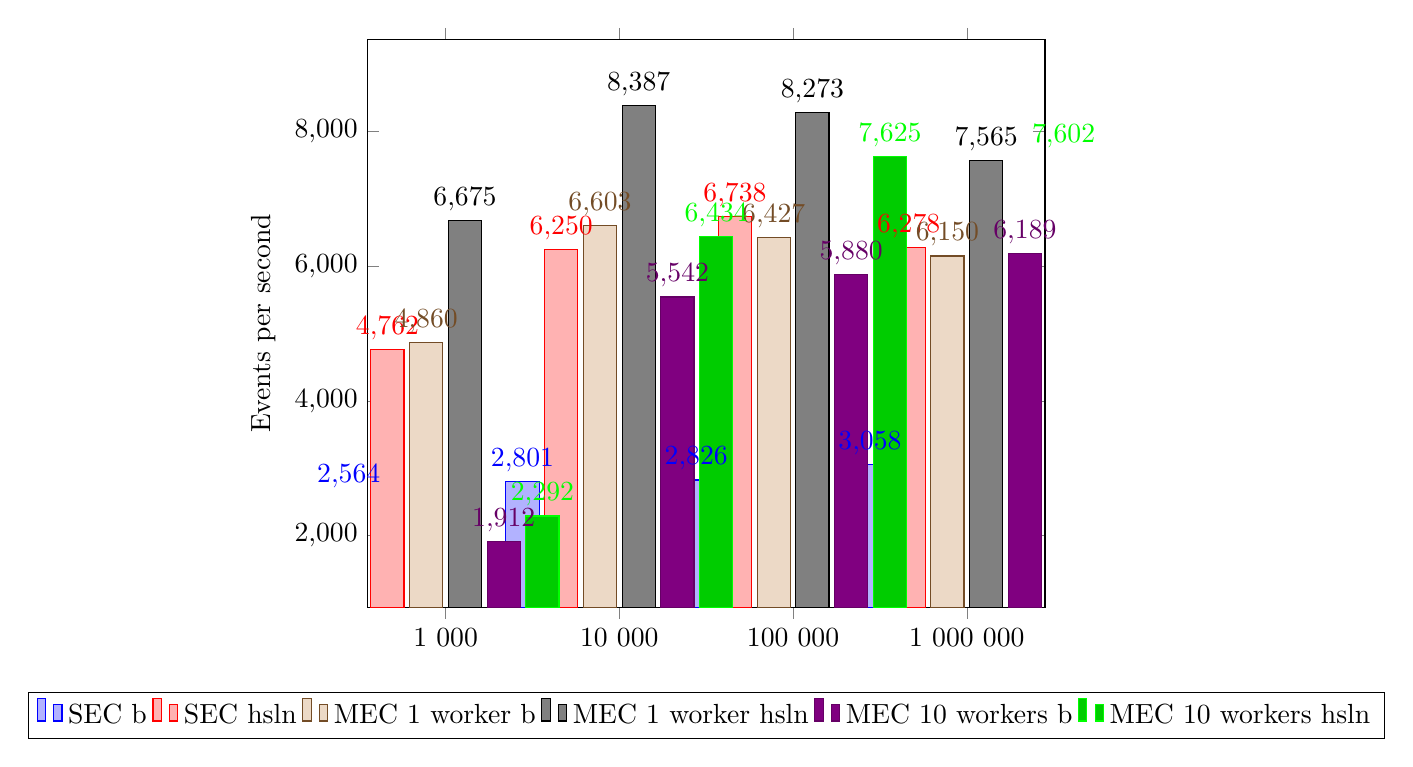
\begin{tikzpicture}
\begin{axis}[
    xtick=data,
	height=250pt,
	ylabel=Events per second,
	enlargelimits=0.15,
	legend style={at={(0.5,-0.15)},
	anchor=north,legend columns=-1},
	ybar,
	bar width=12pt,
	symbolic x coords={1 000, 10 000, 100 000, 1 000 000},
	nodes near coords,
	nodes near coords style={above}
]
\addplot coordinates {(1 000,2564) (10 000,2801) (100 000,2826) (1 000 000,3058)}; % SEC baseline
\addplot coordinates {(1 000,4762) (10 000,6250) (100 000,6738) (1 000 000,6278)}; % SEC high signal low noise

\addplot coordinates {(1 000,4860) (10 000,6603) (100 000,6427) (1 000 000,6150)}; % MEC1W baseline
\addplot coordinates {(1 000,6675) (10 000,8387) (100 000,8273) (1 000 000,7565)}; % MEC1W high signal low noise

\addplot coordinates {(1 000,1912) (10 000,5542) (100 000,5880) (1 000 000,6189)}; % MEC10W baseline
\addplot coordinates {(1 000,2292) (10 000,6434) (100 000,7625) (1 000 000,7602)}; % MEC10W high signal low noise

\legend{SEC b, SEC hsln, MEC 1 worker b, MEC 1 worker hsln, MEC 10 workers b, MEC 10 workers hsln}
\end{axis}
\end{tikzpicture}
\caption{Comparing baseline (b) and High signal low noise (hsln) dataset}
\label{fig:comparing-perf}
\end{figure}

\subsection{Results}
We want to see if our Go implementation can out-perform SEC when handling a high signal, low noise dataset. The Figures \ref{fig:high-signal-low-noise}, \ref{fig:baseline-perf} and \ref{fig:comparing-perf} shows the results for that:
\\

\\
These tests are run with 1 logical core on a "Intel(R) Core(TM) i7-7600U CPU @ 2.80GHz" (2 cores x 2 threads per core = max 4 logical cores) and 24GB RAM.\\
\textbf{What can we say about the performance difference between the two datasets?}\\
It's because of the implementation in SEC and MEC, if we match a rule quickly, we don't have to check all the other rules for a match, and this saves time.\\
\textbf{Why is the MEC10W slower in the start?}\\
Since MEC10W launches ten workers using Go routines, the additional overhead involved with that process is slowing down the performance if you compare it with "single-worker"-style implementations like SEC or MEC with 1 worker.\\
\textbf{Why are the runs on the 1 000 dataset generally lower?}
Because of the small dataset used (1 000), the time spent on general initialization is spread across a lot fewer events, which decreases the events/second throughput.

\subsubsection{Multiple cores}

By using all CPU cores available (4) instead of a single one, we can take better advantage of Gos concurrency model, and raise the throughput when using multiple workers and CPUs as seen in Figure \ref{fig:multicore-hsln-perf} and \ref{fig:multicore-b-perf}.\\
\textbf{What can we say about 1CPU,10W "catching up" to the others around 100 000 events?}\\
This is pretty much the same as what we saw in the single core test.\n{ref her}. The time used to spin up the 10 workers (Go routines) is only outweighed at approximately 100 000 events. This is also why we are seeing a dip when using a dataset of 1 000 events.\\
\textbf{Why are the results of 1CPU,1W, 1CPU,10W and 10CPU,1W generally the same?}\\
This is because they in general are the same. When we are limiting our script to 1 worker, it doesn't really matter how many cores we use, as only one core will be running the worker regardless. There is however a slight benefit to the 4CPU,10W which we can clearly see from the Figure at 1 000 events. The main-function in Go is itself a Go routine, so when we are creating a worker in another core, the main-function can work uninterrupted with reading the log files, while the worker is not blocking since it is running in another core.

\begin{figure}[ht]
\centering
\pgfplotsset{scaled y ticks=false}
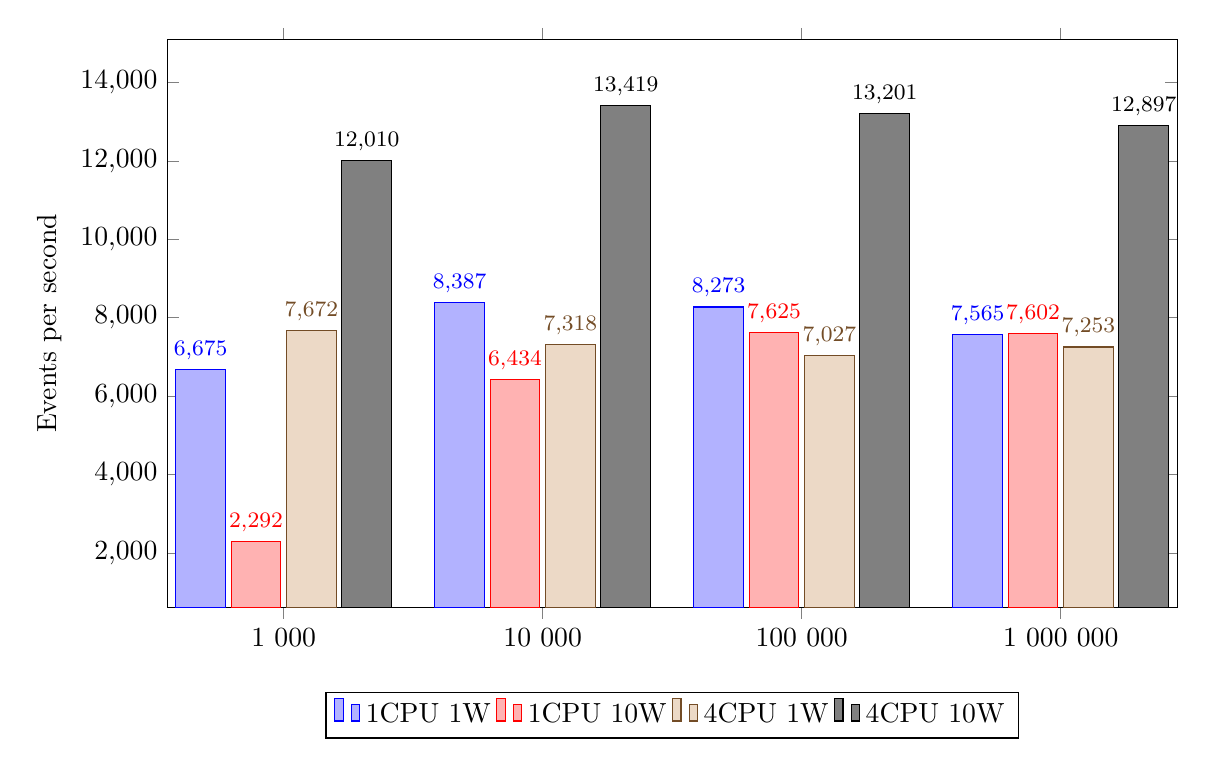
\begin{tikzpicture}
\begin{axis}[
    xtick=data,
    width=410pt,
	height=250pt,
	ylabel=Events per second,
	enlargelimits=0.15,
	legend style={at={(0.5,-0.15)},
	anchor=north,legend columns=-1},
	ybar,
	bar width=18pt,
	symbolic x coords={1 000, 10 000, 100 000, 1 000 000},
	nodes near coords,
	nodes near coords style={above, font=\footnotesize},
]
\addplot coordinates {(1 000,6675) (10 000,8387) (100 000,8273) (1 000 000,7565)}; % 1CPU 1W
\addplot coordinates {(1 000,2292) (10 000,6434) (100 000,7625) (1 000 000,7602)}; % 1CPU 10W
\addplot coordinates {(1 000,7672) (10 000,7318) (100 000,7027) (1 000 000,7253)}; % 4CPU 1W
\addplot coordinates {(1 000,12010) (10 000,13419) (100 000,13201) (1 000 000,12897)}; % 4CPU 10W
\legend{1CPU 1W , 1CPU 10W , 4CPU 1W , 4CPU 10W}
\end{axis}
\end{tikzpicture}
\caption{Concurrency with high signal low noise dataset}
\label{fig:multicore-hsln-perf}
\end{figure}

\begin{figure}[ht]
\centering
\pgfplotsset{scaled y ticks=false}
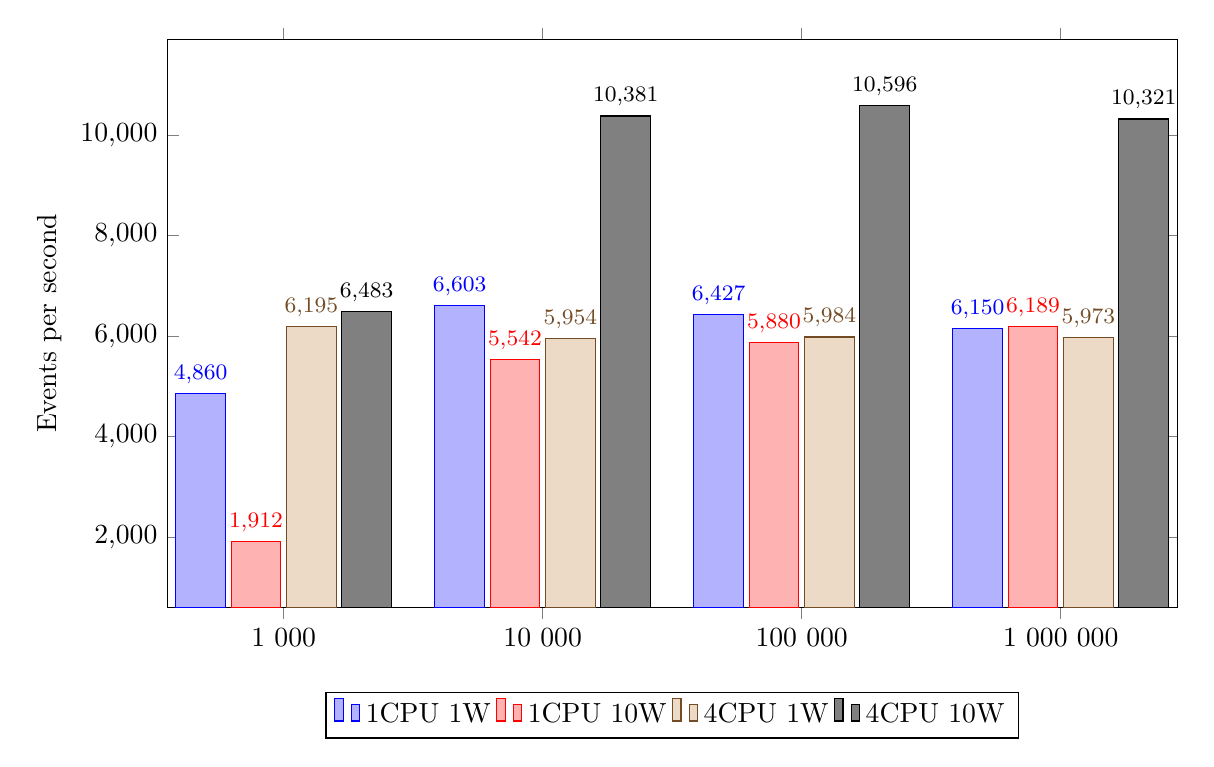
\begin{tikzpicture}
\begin{axis}[
    xtick=data,
    width=410pt,
	height=250pt,
	ylabel=Events per second,
	enlargelimits=0.15,
	legend style={at={(0.5,-0.15)},
	anchor=north,legend columns=-1},
	ybar,
	bar width=18pt,
	symbolic x coords={1 000, 10 000, 100 000, 1 000 000},
	nodes near coords,
	nodes near coords style={above, font=\footnotesize},
]
\addplot coordinates {(1 000,4860) (10 000,6603) (100 000,6427) (1 000 000,6150)}; % 1CPU 1W
\addplot coordinates {(1 000,1912) (10 000,5542) (100 000,5880) (1 000 000,6189)}; % 1CPU 10W
\addplot coordinates {(1 000,6195) (10 000,5954) (100 000,5984) (1 000 000,5973)}; % 4CPU 1W
\addplot coordinates {(1 000,6483) (10 000,10381) (100 000,10596) (1 000 000,10321)}; % 4CPU 10W
\legend{1CPU 1W , 1CPU 10W , 4CPU 1W , 4CPU 10W}
\end{axis}
\end{tikzpicture}
\caption{Concurrency with baseline dataset}
\label{fig:multicore-b-perf}
\end{figure}

\section{Implemented a new rule format}


\subsection{Results}
We are interested in seeing if there are any performance benefits from running our new rule implementation versus the re-implementation of the SEC rules. In the following graph we are running with only a single rule, using our high signal, low noise dataset. The bars labeled "SEC" are our re-implementation of the regular expression-based rules. "Original SEC" is Simple Event Correlator. "MEC" is our implementation with the new rule format.

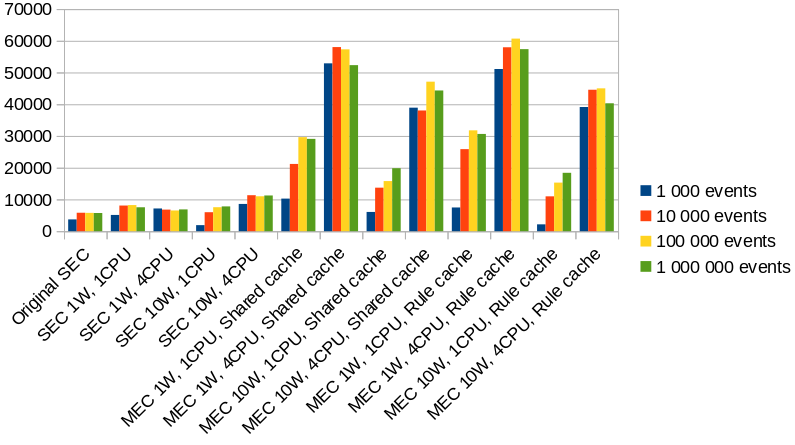
\includegraphics[scale=0.525]{figures/new-rule-format/performance.png}
\\
First of all, we see that our new rule format has in general increased the event throughput substantially. One interesting thing is that there is little to no difference between shared context locking and the rule-based locking in our implementation.

\todo{What happened with 1 000 events for MEC 10W,1CPU rule context locking here?..}

The reason for this could be that we are only using a single rule, so we are not actually benefiting from the different context locking logic that we have implemented. To further explore this, we have generated 1 000 rules randomly, and re-ran our high signal, low noise dataset against them.

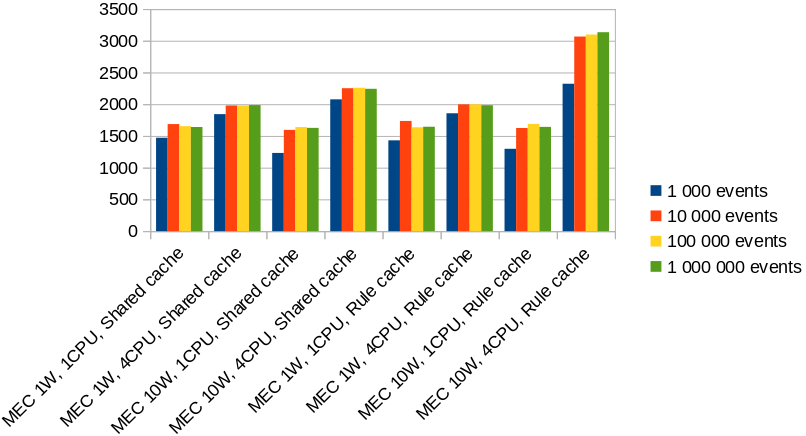
\includegraphics[scale=0.525]{figures/new-rule-format/performance-2.png}
\\
In the above graph, we see a drastic fall in events processed per second, because of the need to iterate over more rules. As expected, we see that rule-cache with 10W and 4CPU gives a 39.77\% increase compared against 10W, 4CPU and shared locking.

What is interesting here is the little difference between (1W, 1CPU), (10W, 1CPU), (1W, 4CPU) and the two different locking implementations. This makes sense, as the low amount of workers don't take advantage of the rule-based context locking, and will then fall to the same speed as shared context locking.

\subsubsection{Low signal, high noise dataset}
\todo{This experiment requires a bit more care. We should discuss context locking method, rules used and why we chose this dataset.}


What happens when we have a low signal, high noise dataset? We can see the result in Figure \ref{fig:comparing-lshn-hsln}. The following experiment explores that. Our hypothesis is that with a dataset where a single rule is triggered only once, we will see a drastic improvement over our high signal, low noise dataset. The reasoning behind this, is that if the events processed do not trigger any of our rules, we can process events much quicker. In addition, if the event does not trigger our rule, the context engine will not come in to play, and we will not have to do any sorts of locking.

This test has been run with a single rule and shared context locking. \n{Discuss why we chose this lock? Should we perhaps try the other as well?}

\begin{figure}[ht]
\centering
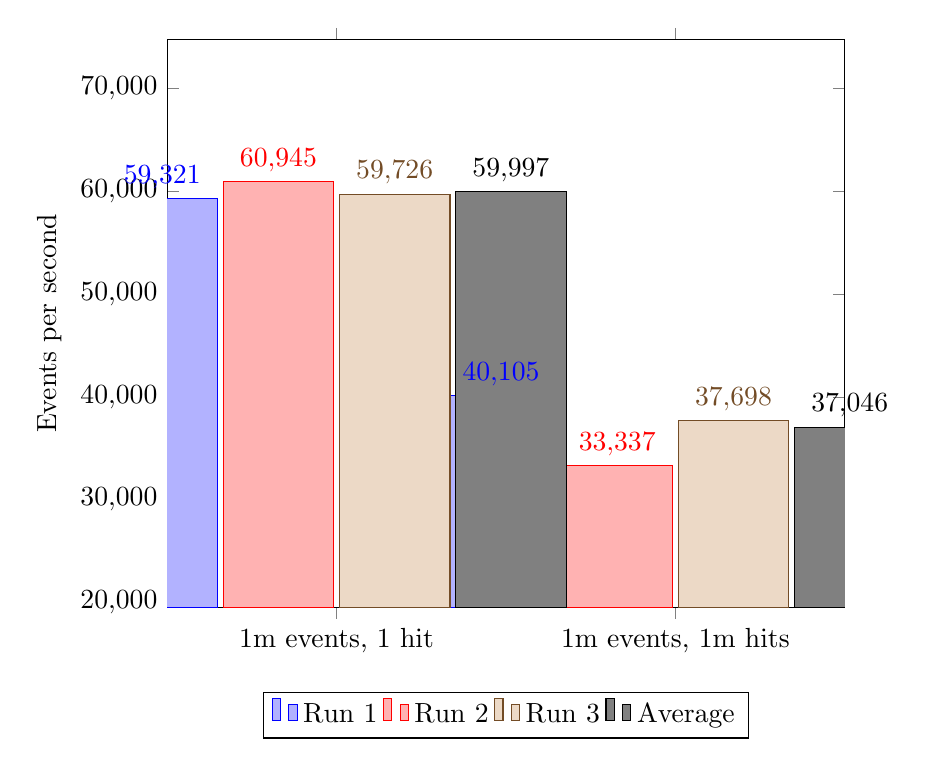
\begin{tikzpicture}
\begin{axis}[
    xtick=data,
	height=250pt,
	ylabel=Events per second,
	enlargelimits=0.5,
	legend style={at={(0.5,-0.15)},
	anchor=north,legend columns=-1},
	ybar,
	bar width=40pt,
	symbolic x coords={{1m events, 1 hit}, {1m events, 1m hits}},
	nodes near coords,
	nodes near coords style={above}
]
\addplot coordinates {({1m events, 1 hit},59321) ({1m events, 1m hits},40105)};
\addplot coordinates {({1m events, 1 hit},60945) ({1m events, 1m hits},33337)};
\addplot coordinates {({1m events, 1 hit},59726) ({1m events, 1m hits},37698)};
\addplot coordinates {({1m events, 1 hit},59997) ({1m events, 1m hits},37046)}; 
\legend{Run 1, Run 2, Run 3, Average}
\end{axis}
\end{tikzpicture}
\caption{Comparing low signal high noise with high signal low noise datasets }
\label{fig:comparing-lshn-hsln}
\end{figure}